\documentclass[xcolor=dvipsnames,table]{beamer}

\usepackage{latexsym}
\usepackage[utf8]{inputenc}
\usepackage[brazil]{babel}
\usepackage{amssymb}
\usepackage{amsmath}
\usepackage{stmaryrd}
\usepackage{fancybox}
\usepackage{datetime}
\usepackage[T1]{fontenc}
\usepackage{graphicx}
\usepackage{graphics}
\usepackage{url}
\usepackage{algorithmic}
\usepackage{algorithm}
\usepackage{acronym}
\usepackage{array}

\usepackage{listings}
\usepackage{color}

\definecolor{mygreen}{rgb}{0,0.6,0}
\definecolor{mygray}{rgb}{0.5,0.5,0.5}
\definecolor{mymauve}{rgb}{0.58,0,0.82}

\lstdefinelanguage{JavaScript}{
  keywords={typeof, new, true, false, catch, function, return, null, catch, switch, var, if, in, while, do, else, case, break},
  keywordstyle=\color{blue}\bfseries,
  ndkeywords={class, export, boolean, throw, implements, import, this},
  ndkeywordstyle=\color{darkgray}\bfseries,
  identifierstyle=\color{black},
  sensitive=false,
  comment=[l]{//},
  morecomment=[s]{/*}{*/},
  commentstyle=\color{purple}\ttfamily,
  stringstyle=\color{red}\ttfamily,
  morestring=[b]',
  morestring=[b]",
}

\lstset{ %
  backgroundcolor=\color{white},   % choose the background color; you must add \usepackage{color} or \usepackage{xcolor}
  basicstyle=\small,        % the size of the fonts that are used for the code
  breakatwhitespace=false,         % sets if automatic breaks should only happen at whitespace
  breaklines=true,                 % sets automatic line breaking
  captionpos=b,                    % sets the caption-position to bottom
  commentstyle=\color{mygreen},    % comment style
  deletekeywords={...},            % if you want to delete keywords from the given language
  escapeinside={\%*}{*)},          % if you want to add LaTeX within your code
  extendedchars=true,              % lets you use non-ASCII characters; for 8-bits encodings only, does not work with UTF-8
  frame=single,	                   % adds a frame around the code
  keepspaces=true,                 % keeps spaces in text, useful for keeping indentation of code (possibly needs columns=flexible)
  keywordstyle=\color{blue},       % keyword style
  language=HTML,                 % the language of the code
  otherkeywords={*,...},           % if you want to add more keywords to the set
  numbers=left,                    % where to put the line-numbers; possible values are (none, left, right)
  numbersep=5pt,                   % how far the line-numbers are from the code
  numberstyle=\tiny\color{mygray}, % the style that is used for the line-numbers
  rulecolor=\color{black},         % if not set, the frame-color may be changed on line-breaks within not-black text (e.g. comments (green here))
  showspaces=false,                % show spaces everywhere adding particular underscores; it overrides 'showstringspaces'
  showstringspaces=false,          % underline spaces within strings only
  showtabs=false,                  % show tabs within strings adding particular underscores
  stepnumber=1,                    % the step between two line-numbers. If it's 1, each line will be numbered
  stringstyle=\color{mymauve},     % string literal style
  tabsize=2,	                   % sets default tabsize to 2 spaces
  title=\lstname,                   % show the filename of files included with \lstinputlisting; also try caption instead of title
  moredelim=**[is][\color{purple}]{@}{@},
}

\newtheorem{definicao}{Definio}
\newcommand{\tab}{\hspace*{2em}}

\mode<presentation>
{
  \definecolor{colortexto}{RGB}{0,0,0}
 
  \setbeamertemplate{background canvas}[vertical shading][ bottom=white!10,top=white!10]
  \setbeamercolor{normal text}{fg=colortexto} 

  \usetheme{Warsaw}
}

\title{Medição} 

\author{
  Esdras Lins Bispo Jr. \\ \url{bispojr@ufg.br}
  } 
 \institute{
  Física para Ciência da Computação \\Bacharelado em Ciência da Computação}
\date{\textbf{26 de agosto de 2019} }

\logo{
\includegraphics[width=1cm]{images/ufgJataiLogo.png}}

\begin{document}

	\begin{frame}
		\titlepage
	\end{frame}

	\AtBeginSection{
		\begin{frame}{Sumário}%[allowframebreaks]{Sumário}
    		\tableofcontents[currentsection]
    		%\tableofcontents[currentsection, hideothersubsections]
		\end{frame}
	}

	\begin{frame}{Plano de Aula}
		\tableofcontents
		%\tableofcontents[hideallsubsections]
	\end{frame}



\section{Medição}
	\begin{frame}{Medindo grandezas}
		\begin{block}{Descobrindo a física...}
			Medindo e comparando grandezas
		\end{block} \pause
		\begin{block}{Grandezas}
			\begin{itemize}
				\item Comprimento, 
				\item Tempo, 
				\item Massa, 
				\item Temperatura, 
				\item Pressão, 
				\item Corrente elétrica...
			\end{itemize}
		\end{block}
	\end{frame}
	
	\begin{frame}{Medindo grandezas}
		\begin{block}{Como medimos uma grandeza}
			Comparando-a com um padrão
		\end{block}	\pause
		\begin{block}{Unidade}
			Medida de uma grandeza
		\end{block} \pause
		\begin{block}{Exemplo}
			Metro é uma unidade de grandeza de comprimento
		\end{block}	
	\end{frame}
	
	\begin{frame}{Medindo grandezas}
		\begin{block}{Sistema Internacional de Unidades (SI)}
			\begin{itemize}
				\item 1971
				\item 14ª Conferência Geral de Pesos e Medidas
				\item Sete grandezas como fundamentais
			\end{itemize}
		\end{block} \pause
		\begin{center}
			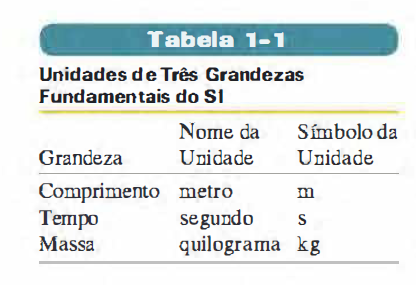
\includegraphics[scale=0.5]{images/tabela1-1.png}
		\end{center}
	\end{frame}
	
	\begin{frame}{Medindo grandezas}
		\begin{block}{Unidades Derivativas}
			São aquelas unidades que podem ser obtidas a partir de unidades fundamentais.
		\end{block} \pause
		\begin{block}{Exemplo}
			1 watt = 1 W = 1 kg $\times m^2 / s^3$
		\end{block}
	\end{frame}
	
	\begin{frame}{Notação Científica}
		\begin{block}{Onde é utilizada?}
			Usa-se a notação científica para expressar as grandezas muito grandes.
		\end{block} \pause
		\begin{block}{Formato}
			\begin{center}
				$a \times 10^b$
			\end{center}
			em que \pause
			\begin{itemize}
				\item $a \in \mathbb{R}$ e $1 \leq a < 10$; e
				\item $b \in \mathbb{Z}^*$.
			\end{itemize}
		\end{block}
	\end{frame}
	
	\begin{frame}{Notação Científica}
		\begin{block}{Exemplos}
			\begin{itemize}
				\item 3.560.000.000 m = $3,56 \times 10^9$ m \pause
				\item 0,000 000 492 s = $4,92 \times 10^{-7}$ s
			\end{itemize}
		\end{block} \pause
		\begin{block}{Em linguagens de programação...}
			A notação abreviada normalmente é usada: \pause
			\begin{center}
				$7.59 e9$ ou $4.93 e-7$
			\end{center}
		\end{block} \pause
		\begin{block}{Umas das utilidades...}
			Bastante útil no processo de conversão de unidades.
		\end{block}
	\end{frame}
	
	\begin{frame}{Uso de prefixos}
		\begin{center}
			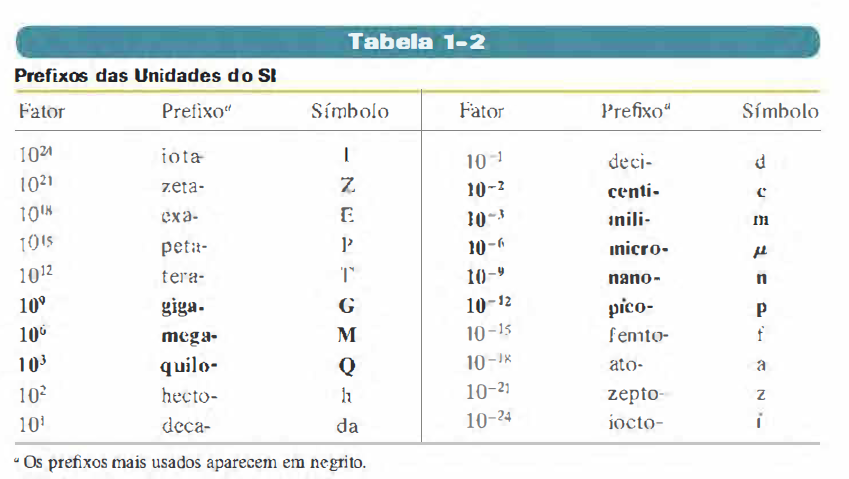
\includegraphics[scale=0.5]{images/tabela1-2.png}
		\end{center}
	\end{frame}
	
	\subsection{Comprimento}
	\begin{frame}{Medida de Comprimento}
		\begin{block}{Comprimento}
			No SI, a unidade para o comprimento é o metro (m).
		\end{block} \pause
		\begin{block}{Metro}
			Distância percorrida pela luz no vácuo durante um intervalo de tempo de 1/299.792.458 de segundo.
		\end{block}
	\end{frame}
	
	\begin{frame}{Curiosidade}
		\begin{center}
			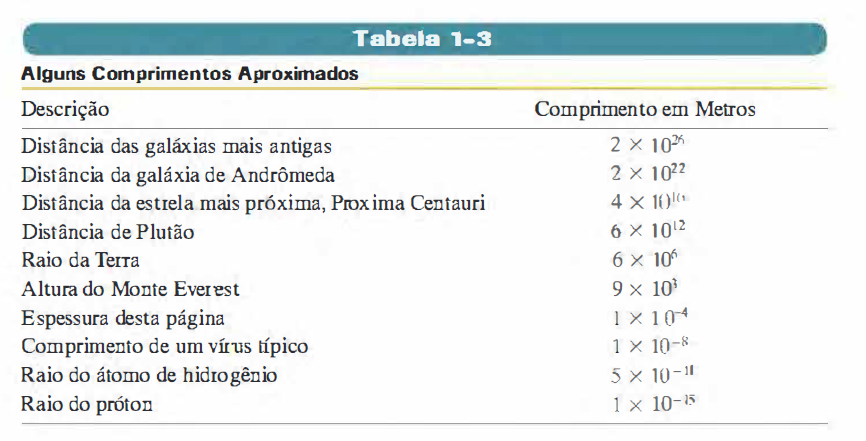
\includegraphics[scale=0.5]{images/tabela1-3.png}
		\end{center}
	\end{frame}
	
	\subsection{Tempo}
	\begin{frame}{Medida de Tempo}
		\begin{block}{Tempo}
			No SI, a unidade para o tempo é o segundo (s).
		\end{block} \pause
		\begin{block}{Segundo}
			O intervalo de tempo que corresponde a 9.192.631.770 oscilações da luz (de um comprimento de onda especificado) emitida por um átomo de césio 133.
		\end{block} \pause
		\begin{block}{Hora Coordenada Universal (UTC)}
			Fornecida por um relógio atômico no Colorado, EUA.
		\end{block}
	\end{frame}
	
	\begin{frame}{Curiosidade}
		\begin{center}
			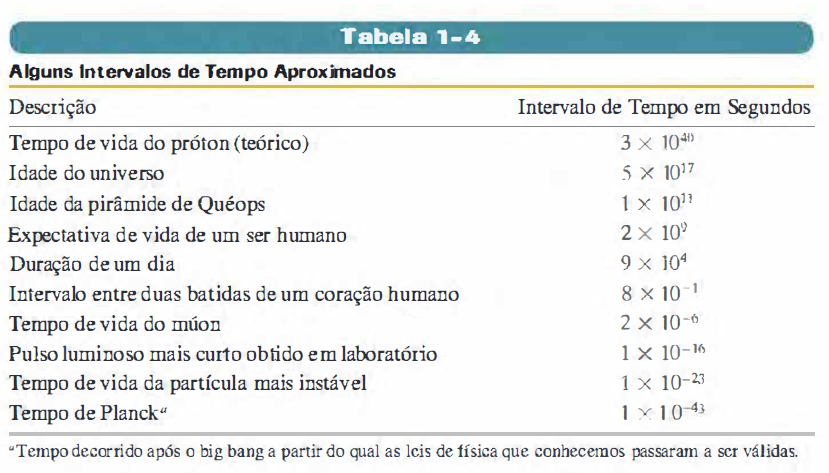
\includegraphics[scale=0.5]{images/tabela1-4.png}
		\end{center}
	\end{frame}
	
	\subsection{Massa}
	\begin{frame}{Medida de Massa}
		\begin{block}{Massa}
			No SI, a unidade para massa é o quilograma (kg).
		\end{block} \pause
		\begin{block}{Quilograma}
			Um cilindro de platina irídio com 3,9cm de altura e 3,9cm de diâmetro.
		\end{block} \pause
		\begin{center}
			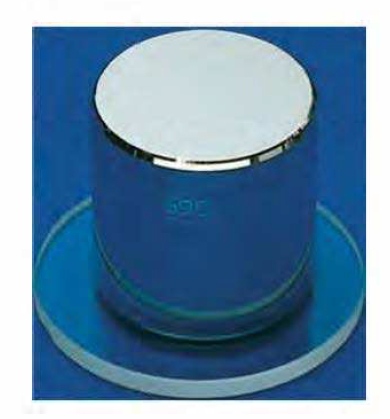
\includegraphics[scale=0.3]{images/figura1-3.png}
		\end{center}
	\end{frame}
	
	\begin{frame}{Curiosidade}
		\begin{center}
			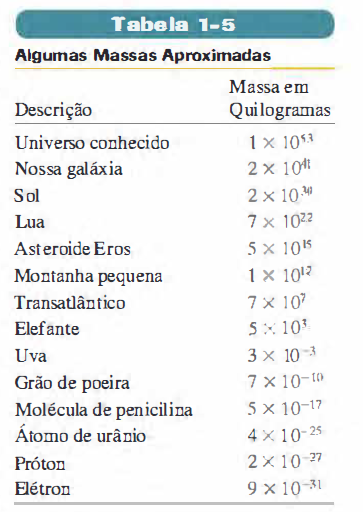
\includegraphics[scale=0.5]{images/tabela1-5.png}
		\end{center}
	\end{frame}	
	
	\begin{frame}{Massa Específica}
		\begin{block}{Massa específica}
			É a massa por unidade de volume.
			\begin{center}
				$\rho = \dfrac{m}{V}$
			\end{center}
		\end{block} \pause
		\begin{block}{Exemplo: Massa específica da água}
			1 g/$\mbox{cm}^3$
		\end{block}
	\end{frame}
	
	\begin{frame}[shrink]{Bônus}
		\begin{block}{Desafio}
			{\bf (Halliday 2.68)} Em um soco direto de caratê, o punho começa em repouso na cintura e é movido rapidamente para a frente até o braço ficar completamente estendido. A velocidade $v(t)$ do punho está representada na figura (próximo slide) para o caso de um lutador experiente. A escala vertical é definida por $v_s = 8,0 m/s$. Qual é a distância percorrida pelo punho desde o início do golpe até
			\begin{enumerate}
				\item o instante t = 50 ms, e 
				\item o instante em que a velocidade do punho é máxima?
			\end{enumerate} 
		\end{block} \pause
		\begin{block}{Informações úteis}
			\begin{itemize}
                \item Candidaturas (28 de agosto, 17h20);
                \item Resposta escrita e apresentação (04 de setembro, 18h30).
			\end{itemize}
		\end{block} 
	\end{frame}
	
	\begin{frame}{Bônus (0,5 pt)}
		\begin{center}
			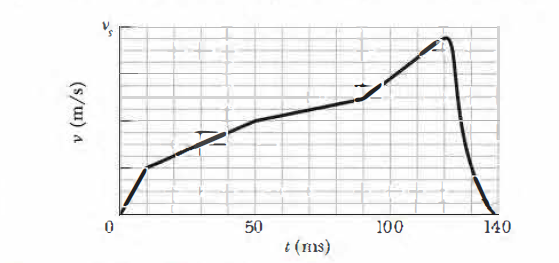
\includegraphics[scale=0.5]{images/bonus.png}
		\end{center}
	\end{frame}
	
	\begin{frame}
		\titlepage
	\end{frame}
	
\end{document}